\begin{frame}
\frametitle{Virtualbox NAT}
	\begin{columns}
	\column{0.5\textwidth}
        \begin{itemize}
            \item Встроенный DHCP сервер
            \item Доступ в Internet
            \item Доступ из хост системы (только через проброс портов)
        \end{itemize}
	\column{0.5\textwidth}
    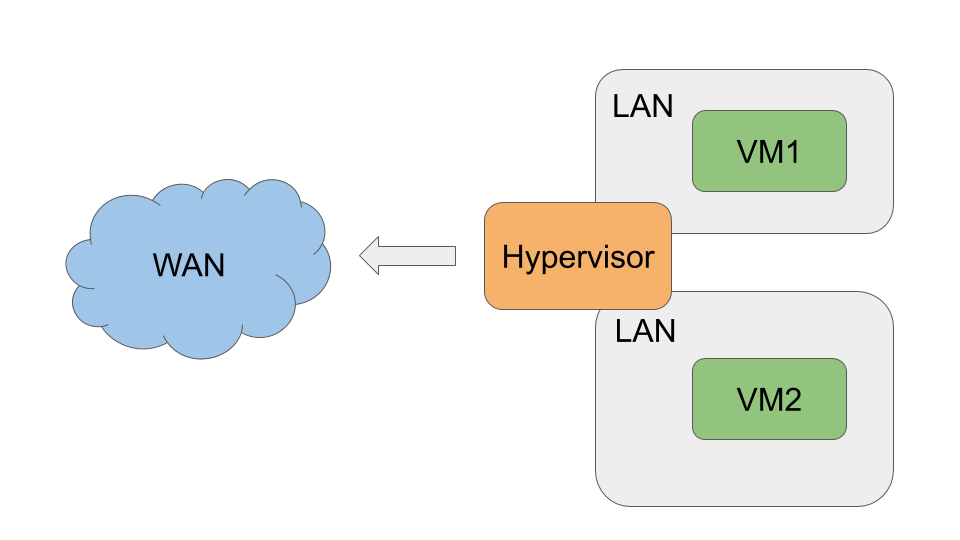
\includegraphics[height=0.4\textheight]{../../slides/vbox/Virtualbox network NAT.png}
    \end{columns}
    10.0.2.15 - IP адрес, выданный в этом режиме.
\end{frame}